\documentclass{beamer}
\usetheme[titleformat=regular,sectiontitleformat=regular,frametitleformat=regular]{m}

\usepackage[noend]{algpseudocode}
\usepackage{algorithm}

\usepackage[brazil]{babel}
\usepackage[numberedbib]{apacite}
\usepackage[utf8]{inputenc}
\usepackage{mathabx}
\usepackage{tabularx}
\usepackage{lipsum}
\usepackage{multicol}

\newcommand\Fontvi{\fontsize{7}{7.2}\selectfont}


\title{Programação automática evolucionária aplicada ao problema de deduplicação de registros}
\date{\today}
\author{Acadêmico: Herberth Amaral \\
Orientador: Prof. Dr. Renê Rodrigues Veloso}
\institute{Programa de Pós-Graduação em Modelagem Computacional e Sistemas - UNIMONTES}
\begin{document}
  \maketitle

  \section{Problema}

  \begin{frame}{Problema}
      \begin{itemize}
          \item Duplicação de registros é um problema de qualidade de bases de dados;
          \item Instituições com diferentes softwares para diferentes problemas;
          \item Várias bases de dados;
          \item Registros duplicados entre bases de dados;
      \end{itemize}
  \end{frame}

  \begin{frame}{Exemplo de duplicação de registros em uma instituição de saúde}
      \begin{figure}
          \centering
          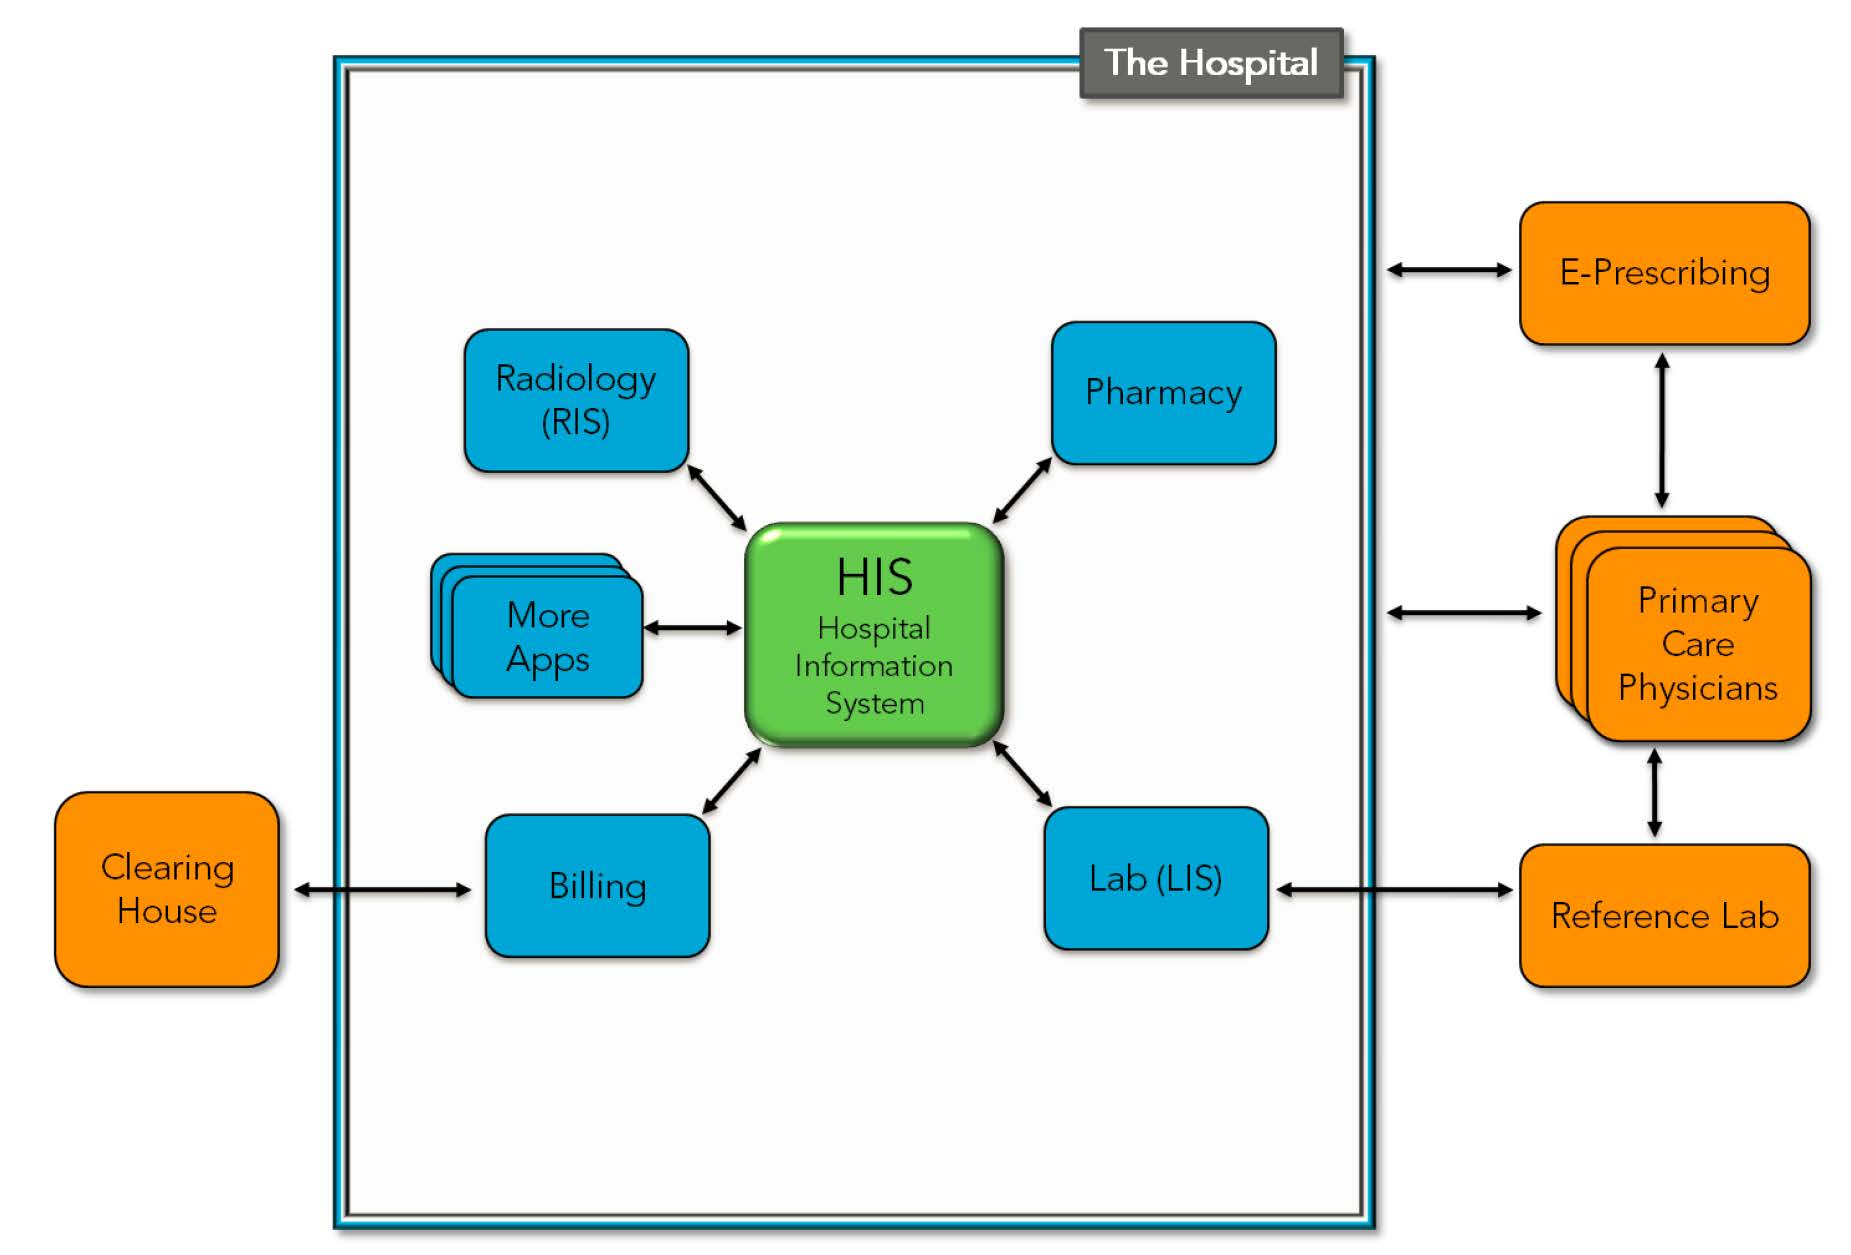
\includegraphics[width=1.0\textwidth]{hospital.jpg}
          \caption{Diferentes sistemas dentro de um hospital \cite{hospital}}
      \end{figure}
  \end{frame}

  \begin{frame}{Problemas com registros duplicados}
      Os principais problemas com registros duplicados/distribuídos em uma instituição de saúde são:
      \begin{itemize}
          \item Impossibilidade de unificação de prontuários de forma confiável;
          \item Dificuldades de comunicação entre diferentes setores (ex: farmácia e financeiro);
          \item Erros de diagnóstico;
          \item Falta de confiança em processos informatizados.
      \end{itemize}
  \end{frame}

  \section{Deduplicação de registros}

  \begin{frame}{Introdução à deduplicação de registros}
      \begin{itemize}
          \item Deduplicação de registros (também conhecido como \textit{record linkage - RL}) é o processo de identificação de registros duplicados que representam a mesma entidade em um ou mais bases de dados \cite{survey};
          \item Permite a unificação de dados a partir de um ponto em comum (ex: paciente).
      \end{itemize}
  \end{frame}

  \begin{frame}{Processo de deduplicação}
      \begin{figure}
          \centering
          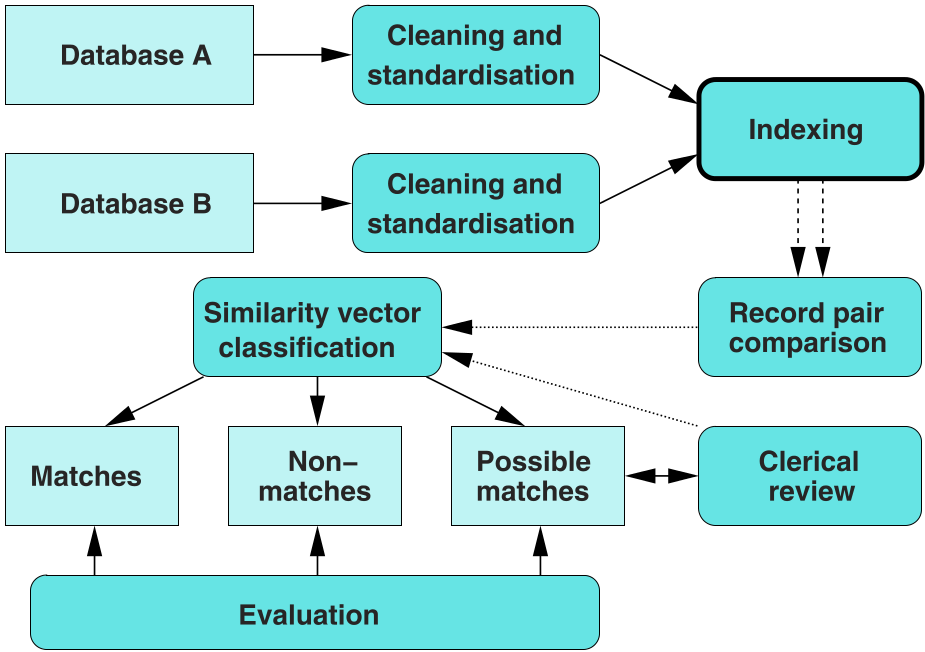
\includegraphics[width=0.9\textwidth]{rlprocess.png}
          \caption{Processo de deduplicação \cite{survey}}
      \end{figure}
  \end{frame}

  \begin{frame}{Funções de similaridade para comparação de registros}
      \begin{table}
          \centering
          \caption{Algumas funções de similaridade \cite{survey}}
          \begin{tabularx}{\textwidth}{|l|X|}
              \hline
              Função                    & Observação \\ \hline
              Jaro                      & Principalmente para primeiros e últimos nomes. Retorna um valor no intervalo $[0,1]$ em que 0 é diferente e 1 é igual. \cite{jaro}\\ \hline
              Jaro-Winkler              & Baseado na Jaro. Dá mais pesos à prefixos. \cite{jaro-winkler} \\ \hline
              Levenshtein               & Número de edições entre duas strings. 0 significa que são iguais\\ \hline
              Similaridade de cosenos   & Intervalo $[-1, 1]$. Utilizado em busca em textos. \\ \hline
          \end{tabularx}
      \end{table}
  \end{frame}

  \begin{frame}{Breve exemplo}
      Considere dois bancos de dados de exemplo:
      \Fontvi
      \begin{multicols}{2}
          \begin{table}[]
              \centering
              \caption{Banco de dados A}
              \begin{tabular}{|l|l|l|l|}
                  \hline
                  ID & Nome  & Sobrenome & Nascimento \\ \hline
                  1  & Luís  & Silva     & 1990-05-01 \\
                  2  & Marco & Túlio     & 1978-03-14 \\ \hline
              \end{tabular}
          \end{table}
          \columnbreak
          \begin{table}[]
              \centering
              \caption{Banco de dados B}
              \begin{tabular}{|l|l|l|l|}
                  \hline
                  ID & Nome   & Sobrenome & Nascimento \\ \hline
                  1  & Luiz   & Silva     & 1990-01-05 \\
                  2  & Marcos & Tulio     & 1978-03-14 \\
                  3  & Pedro  & Ferreira  & 1989-10-21 \\ \hline
              \end{tabular}
          \end{table}
      \end{multicols}

      \textbf{Problema:} Como descobrir as duplicatas?
  \end{frame}

  \begin{frame}{Comparação campo-a-campo}
      \begin{table}[]
          \centering
          \caption{Comparação entre dois registros das bases de dados (depois da limpeza)}
          \label{tbl:comparacao}
          \begin{tabular}{|l|l|l|l|}
              \hline
              Função de comparação             & Nome & Sobrenome & Nascimento \\ \hline
              Jaro                             & luiz & silva     & 1990-05-01 \\
              Jaro                             & luis & silva     & 1990-01-05 \\ \hline
              \textbf{Resultado da comparação} & 0.83 & 1         & 0.96       \\ \hline
          \end{tabular}
      \end{table}

      Chamaremos de $E$ o vetor resultante da comparação.
  \end{frame}
  \begin{frame}{Regra de ligação (classificação)}
      Função que associa o vetor de comparação $E$ com a probabilidade do par de registros pertencerem a uma mesma entidade.

      \textbf{Exemplo:} \[
          F_s(E) = \begin{cases}
              1  &  \text{if }\dfrac{\sum \limits_{e \in E} e}{|E|} \geq 0.95 \\
              0  &  \text{otherwise} \\
          \end{cases}
      \]

      \textbf{Problema:} infelizmente, nem sempre a regra de ligação é tão simples.
  \end{frame}

  \section{Objetivos}
  \begin{frame}{Objetivo geral}
      Desenvolver uma melhoria para o trabalho desenvolvido em \cite{geneticrl} através do uso de programação automática por formigas (DAP) em detrimento à programação genética (GP).
  \end{frame}
  \begin{frame}{Objetivos específicos}
      \begin{itemize}
          \item Um algoritmo de programação genética eficiente do ponto de vista de melhores ajustes de regras de ligação;
          \item Extensões de algoritmos para comparação de pares de registros em meio a dados faltantes;
          \item Uma métrica similar a Jaro-Winkler para nomes lusófonos.
      \end{itemize}
  \end{frame}

  \section{Proposta deste trabalho: DAP para geração das regras de ligação}
  \begin{frame}{\textit{Dynamic ant programming}}
      \begin{itemize}
          \item Programação genética (\textit{Genetic programming - GP}) é uma técnica proposta por \cite{koza} para evolução artificial de programas de computador;
          \item Problema do inchaço;
          \item Programação automática por formigas (\textit{Dynamic ant programming - DAP}) é uma forma de geração automática de programas que resolve o problema do inchaço através da limitação prévia do número de nós \cite{shirakawa}.
      \end{itemize}
  \end{frame}

  \begin{frame}{Algoritmo}
        \begin{algorithm}[H]
        \caption{Dynamic Ant Programming}
        \label{alg:dap}
        \begin{algorithmic}[1]

        \Procedure{DAP}{m:numero de formigas}
        \Repeat
        \For{k=1 \textbf{to} m}
        \Repeat
          \State{Do nó atual $i$, selecione o nó $j$ com probabilidade definida na eq.\ref{eq:pkijt}}
        \Until{caminho completo ser construido}
        \EndFor
        \State Atualiza feromônio utilizando eq.\ref{eq:atualizacao-feromonio}
        \State{Exclui nós;}
        \State Insere nós;
        \Until{condição de parada é verdadeira}
        \EndProcedure
        \end{algorithmic}
        \end{algorithm}
  \end{frame}

  \begin{frame}{Funcionamento do DAP}
      A probabilidade da formiga $k$ localizada no nó $i$ movendo do nó $j$ para o nó $u$ no tempo $t$ é:
      \begin{equation}
          \label{eq:pkijt}
          p^k_{i_uj}(t) = \begin{cases}
              \dfrac{\tau_{i_uj}(t)}{\sum_{l\in N^k_i(t)}\tau_{i_ul}(t)} & \text{ if } j \in N^k_i(t) \\
              0 & \text{ if } j \notin N^k_i(t) \\
          \end{cases}
      \end{equation}

      A atualização de feromônio é feita segundo a seguinte regra:

      \begin{equation}
          \label{eq:atualizacao-feromonio}
          \tau_{ij}(t+1) = (1-\rho)\tau_{ij}(t) + \Delta\tau^{best}_{ij}(t), \rho \in (0,1]
      \end{equation}

      $\Delta\tau^{best}_{ij}$ é definido da seguinte forma:

      \begin{equation}
          \label{eq:delta-t}
          \Delta\tau^{best}_{ij}(t) = \begin{cases}
              \dfrac{Q}{L_k} & \text{ if} (i,j) \in T_k \\
              0 & \text{ otherwise}
          \end{cases}
      \end{equation}
  \end{frame}

  \begin{frame}{Metodologia deste trabalho}
      \begin{itemize}
          \item Baseia-se primeiramente na metodologia em \cite{geneticrl};
          \item Substitui a evolução de programas usando programação genética (GP) pela técnica de progrmação automática por formigas (DAP);
          \item \textit{Hipótese}: programas menores e mais expressivos, sem perda da capacidade de generalização;
      \end{itemize}
  \end{frame}

  \begin{frame}{Função de \textit{fitness}}
      Utiliza-se o escore F1, uma média harmônica entre \textit{precisão}
      (chance de acontecer uma classificação correta) e \textit{revocação}
      (chance de uma classificação positiva dela ser realmente positiva).
      Matematicamente falando:
      \begin{equation}
          P = \dfrac{T_p}{T_p+F_p}
      \end{equation}
      \begin{equation}
          R = \dfrac{T_p}{T_p+F_n}
      \end{equation}
      \begin{equation}
          \label{eq:f1-score}
          F_1 = 2\cdot \dfrac{P\cdot R}{P+R}
      \end{equation}
  \end{frame}

  \begin{frame}{Resultados parciais}
      Parâmetros:
        \begin{itemize}
            \item \textbf{População:} 20 formigas;
            \item \textbf{Gerações:} 20 gerações;
            \item \textbf{Critério de parada:} finalização das 20 gerações;
            \item \textbf{$\tau_{min}$:} 0;
            \item \textbf{$\tau_{max}$:} 1;
            \item \textbf{$\rho$:} 0.5;
            \item \textbf{Métrica de fitness:} Escore F1;
        \end{itemize}
  \end{frame}

  \begin{frame}{Resultados parciais}
    Dentre as execuções, o melhor valor final do escore F1 foi 0.9821, com uma média de 0.8412 ($\sigma=0.1691$) e mediana 0.8844.
    \begin{figure}[H]
        \centering
        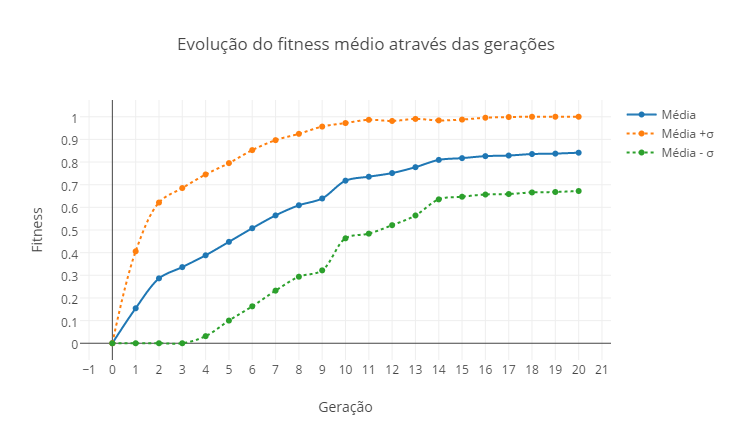
\includegraphics[width=0.8\textwidth]{grafico.png}
        \caption{Evolução do fitness médio e respectivo desvio padrão através das gerações}
        \label{fig:grafico}
    \end{figure}
  \end{frame}

  \begin{frame}{Resultados parciais}
        \begin{table}[H]
        \centering
        \caption{Comparação entre o método proposto por \cite{geneticrl} e método por DAP}
        \label{tbl:comparacao}
        \begin{tabular}{ll}
        \multicolumn{1}{c}{\textbf{Média GP (DP)}} & \multicolumn{1}{c}{\textbf{Média DAP (DP)}} \\
        0.956 (0.053)                                & 0.841 (0.169)
        \end{tabular}
        \end{table}
  \end{frame}


  \section{Conclusões e direcionamento de pesquisa}
  \begin{frame}{Conclusões}
      \begin{itemize}
          \item Proposta apresentada em estágio inicial, outra proposta em desenvolvimento;
          \item Resultados estatisticamente equivalentes àqueles apresentados por \cite{geneticrl};
      \end{itemize}
  \end{frame}
  \begin{frame}{Direcionamento de pesquisa}
      \Fontvi
      \begin{itemize}
          \item Usar outras abordagens para inserção e remoção de nós;
          \item Outras abordagens em colônia de formigas (evaporação de feromônio, escolha de nó, etc);
          \item Adaptação da função Jaro-Winkler para o contexto local;
      \end{itemize}
  \end{frame}

  \begin{frame}{Cronograma}
      \begin{figure}
          \centering
          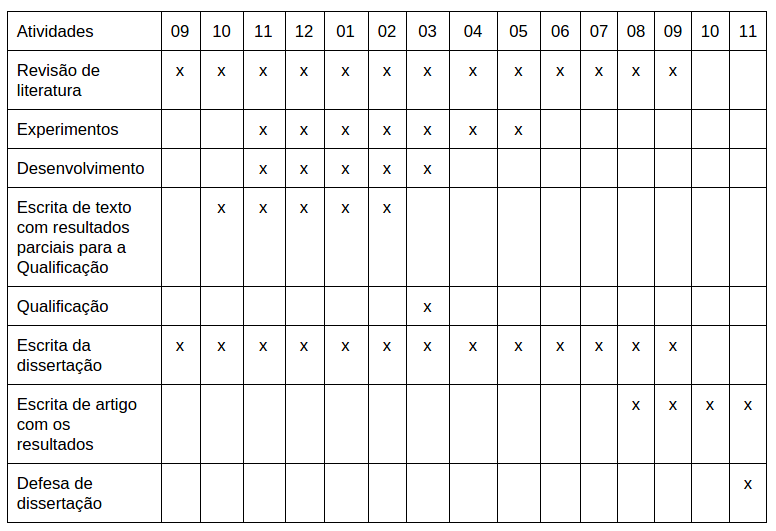
\includegraphics[width=0.9\textwidth]{cronograma.png}
      \end{figure}
  \end{frame}

  \section{Perguntas}
  \section{Muito obrigado!}
  \begin{frame}{Códigos}
      Os códigos dos experimentos feitos até agora estão disponibilizados em \url{https://github.com/herberthamaral/mestrado/tree/master/ProjetoDissertacao}.
  \end{frame}

  \begin{frame}
      \bibliographystyle{apacite}
      \bibliography{apresentacao}
  \end{frame}
\end{document}
